\section{Results}
\label{sec:results}
All 240 fits completed and passed the technical checks. Within every block, the four conditions started from identical weights, B/F and C/R pairs drew identical patch sequences, and the loss targets matched the paired imbalanced allocation. The balanced reference B and condition R reproduce the cross-entropy runs of the mitigation studies: B is 36.49 on BRACS and 71.45 on TCGA-UT (earlier 36.53 and 71.51), and total damage is 5.07 and 1.58 percentage points (earlier 4.95 and 1.56). Table~\ref{tab:results} lists all accuracies and contrasts; Figure~\ref{fig:components} shows the contrasts with their intervals.

\begin{table}[htbp]
\centering
\small
\renewcommand{\arraystretch}{1.15}
\begin{tabular}{@{}lll@{}}
\csname @@input\endcsname arm_table.tex
\end{tabular}
\caption{Coverage-only damage accounts for most estimated BRACS damage; the interaction accounts for most on TCGA-UT, where both single-factor intervals span zero. Rows one to four are patient-macro balanced accuracies (\%); the remaining rows are contrasts in percentage points, with positive damage meaning lower accuracy under imbalance. Brackets give 95\% paired bootstrap intervals.}
\label{tab:results}
\end{table}

\begin{figure}[htbp]
\centering
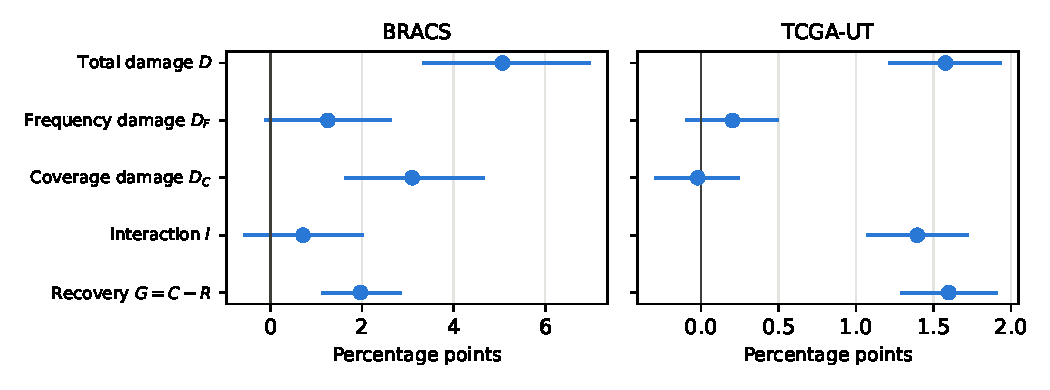
\includegraphics[width=\textwidth]{component_figure.pdf}
\caption{Damage components at $\rho=100$ under low-rank adaptation (LoRA), with 95\% paired intervals. On BRACS, coverage-only damage is the only resolved component besides the total; on TCGA-UT, the interaction is resolved and both single-factor damages are close to zero. The horizontal scales differ between panels.}
\label{fig:components}
\end{figure}

\paragraph{BRACS.} Training on the imbalanced patches with balanced class influence costs 3.09 [1.62, 4.67] points, about three-fifths of the total damage of 5.07 [3.32, 6.98]. Skewing class influence on the balanced patches costs 1.26 [$-0.13$, 2.64] points, and the interaction is 0.72 [$-0.58$, 2.03]; neither interval excludes zero. Restoring balanced class influence on the imbalanced patches recovers $G = 1.97$ [1.12, 2.87] points, a share $h = 0.39$ [0.24, 0.56] of total damage. The share meets the interpretation criteria: total damage exceeds one point and its interval lies above zero. No bootstrap replicate has a non-positive denominator. Across the three splits, coverage-only damage ranges from 2.69 to 3.77 points and the share from 0.36 to 0.42.

\paragraph{TCGA-UT.} Both single-factor damage estimates are close to zero and their intervals span zero: frequency-only damage is 0.20 [$-0.10$, 0.50] and coverage-only damage is $-0.02$ [$-0.30$, 0.25] points. Together they cost 1.58 [1.21, 1.94] points, with the interaction of 1.40 [1.07, 1.73] accounting for most of the estimated damage. Restoring balanced class influence recovers $G = 1.60$ [1.29, 1.91] points, a share $h = 1.01$ [0.86, 1.22] of the damage. The share interval includes full recovery but also allows incomplete recovery or recovery beyond the balanced reference. The coverage-only interval spans small gains and losses rather than establishing exact equality. Across the three splits, the interaction ranges from 1.30 to 1.55 points and the share from 0.95 to 1.08.

\paragraph{Sources of uncertainty.} Resampling only patients or only draws gives intervals of similar width, both narrower than the full intervals. On BRACS, for example, frequency-only damage has a patient-only interval of [0.62, 1.94] and a draw-only interval of [0.15, 2.34]; on TCGA-UT, the interaction has corresponding intervals of [1.23, 1.56] and [1.15, 1.63]. Uncertainty therefore comes from both the finite test cohort and variation between allocation draws, which here also includes random initialization.

\paragraph{Comparison with the frozen readout.} The decomposition differs from that of the frozen-encoder logistic-regression readout on the same patients \citep{queisler2026causeBracs,queisler2026causeTcga}, mainly in frequency-only damage. On BRACS, the frozen readout lost 4.47 points to frequency and 3.29 to coverage; under LoRA, frequency-only damage falls to 1.26, while coverage-only damage remains similar at 3.09. On TCGA-UT, the frozen readout lost 1.20 points to frequency, 0.53 to coverage, and 1.18 to the interaction; under LoRA, both single-factor damage estimates are close to zero, while an interaction of similar size, 1.40, remains. The two learners also differ in loss, optimizer, and training length, so this comparison does not isolate an effect of LoRA.

\paragraph{Comparison with the mitigation methods.} Figure~\ref{fig:recovery} compares recoveries from the mitigation studies with the benchmark $G$. These recoveries use the earlier runs and their own estimate of total damage, so the comparison is descriptive. On BRACS, training-time and post-hoc logit adjustment recover 1.96 and 1.94 points, close to $G = 1.97$. Curriculum of data augmentation (CUDA) recovers more, 2.59 points, but subtracting its gain on balanced data leaves only 1.20 points, below the benchmark in point estimate. On TCGA-UT, training-time and post-hoc logit adjustment recover 1.54 and 1.41 points, within the interval for $G = 1.60$. The estimates are descriptively similar to the benchmark; this comparison does not establish equal recovery.

\begin{figure}[htbp]
\centering
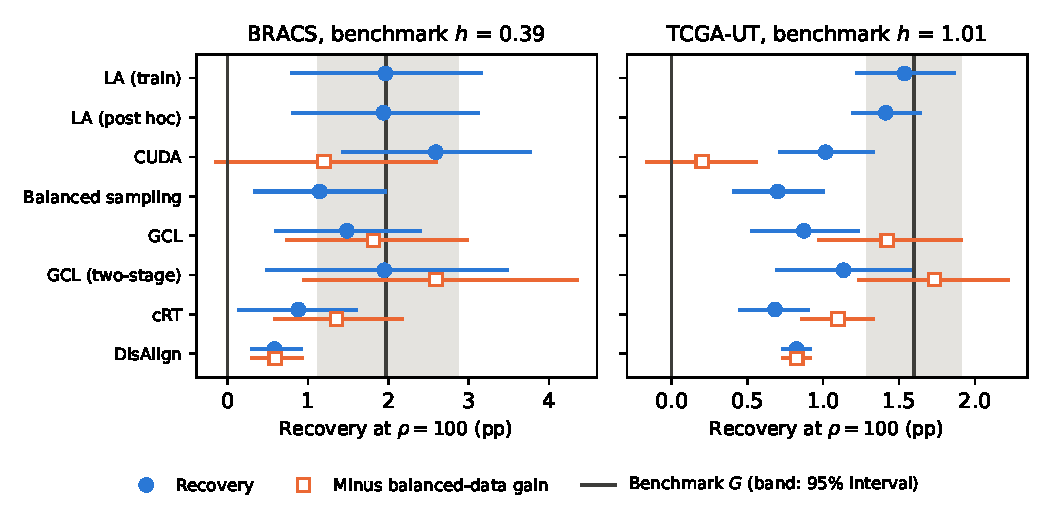
\includegraphics[width=\textwidth]{recovery_figure.pdf}
\caption{Logit adjustment gives descriptively similar recovery to restoring balanced class influence on both datasets. Points show each mitigation method's recovery at $\rho=100$ from the mitigation studies (filled) and, where defined, the recovery after subtracting its gain on balanced data (open). The vertical line and band show this experiment's benchmark $G$ and its 95\% interval; the panel titles give the share $h=G/D$. Method abbreviations: LA, logit adjustment; CUDA, curriculum of data augmentation; GCL, Gaussian clouded logit adjustment; cRT, classifier re-training.}
\label{fig:recovery}
\end{figure}

\section{Discussion}
\label{sec:discussion}
Under the LoRA recipe of the mitigation studies, restoring balanced class influence recovers about two-fifths of the BRACS damage and leaves about three points unrecovered. On TCGA-UT, both single-factor damage estimates are close to zero and the interaction accounts for most estimated damage. The coverage-only interval spans small gains and losses, consistent with full recovery.

Logit adjustment recovered close to $G$: about two-fifths of the BRACS damage and nearly all of the TCGA-UT damage. This fits the conditional statement of Section~\ref{sec:interpretation}: a method that removes frequency-related damage while leaving the coverage-only residual unchanged should recover close to $G$. The agreement is descriptive, follows already known mitigation results, and does not establish a shared mechanism with loss reweighting. The BRACS residual concerns uniform loss reweighting under this fixed recipe; whether another weighting scheme, objective, or training recipe could reduce it remains untested by the decomposition.

The comparison with the frozen readout cautions against transferring earlier shares. Frequency-only damage was the largest BRACS component under the frozen readout; coverage-only damage is largest under LoRA. A share estimated for one learner therefore does not carry over to another learner on the same data, motivating the repeated decomposition.
